%In the following, we 

%\color{blue}




%\revised{:q

In this section, we report how \CT has been evaluated, having the {\em goal} of evaluating the performance of the proposed approach. In Section~\ref{sec:Dataset}, the dataset involved in our evaluation has been presented. We describe the evaluation methodology and metrics in Section~\ref{sec:methodology-metric}. Finally, Section~\ref{sec:ResearchQuestions} describes the research questions.


%ten equal parts, so-called folds
%We also exploited 
%was also exploited 

\begin{figure*}[h!]
	\centering
	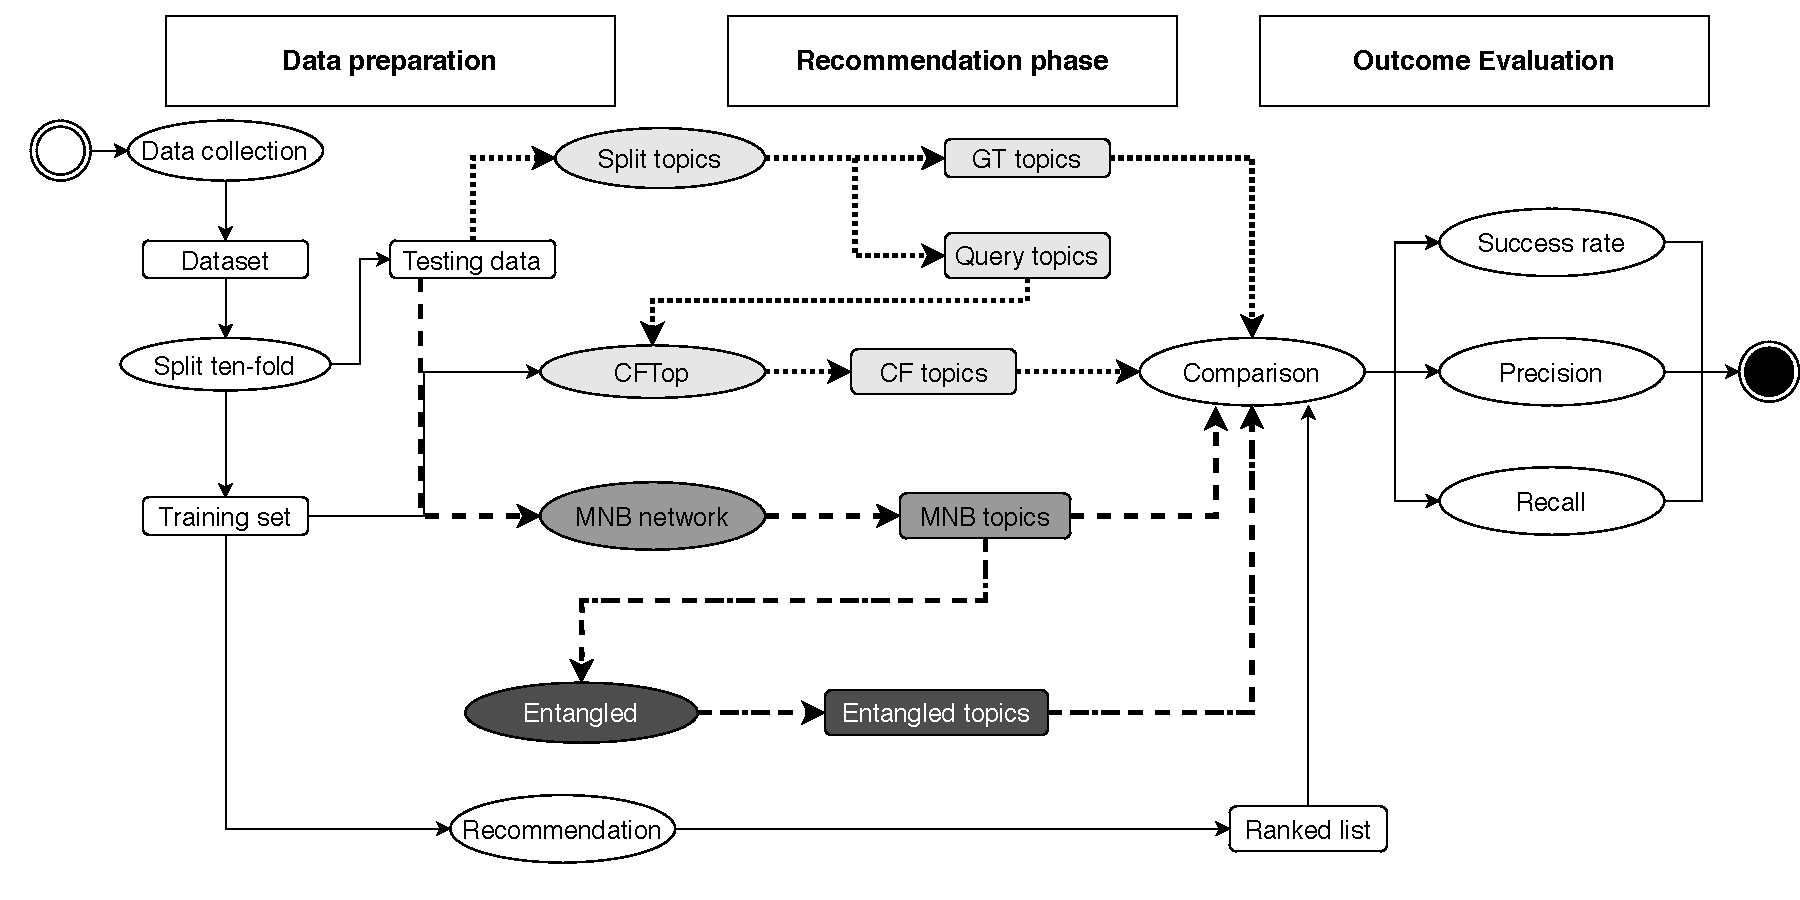
\includegraphics[width=0.9\linewidth,keepaspectratio]{figs/evaluationCF.pdf}
	%\vspace{-.3cm}
	\caption{Evaluation Process.}
	\label{fig:EvaluationProcess}
	\vspace{-.3cm}
\end{figure*}

\subsection{Dataset Extraction} \label{sec:Dataset}


%\color{blue}

To evaluate the approach, we reuse the same dataset employed for the \MNB available here \cite{MNBreplication}. The \GH query language \cite{understanding} allows the fetching of relevant repository metadata including name, owner, and list of topics to mention a few. Thus, we \emph{randomly} collected a dataset consisting of $6,258$ repositories that use 15757 topics by means of the GitHub API \cite{pygithub/pygithub_2019}. To overcome the request limit during the crawling activity, we employ the \GH star voting mechanism as a popularity measure \cite{borges_whats_2018}. As claimed in several works\cite{borges_popularity_2017, borges_predicting_2016}, a high number of stars means the attention of the community for that project. So, we impose the following filter during the query execution:
\begin{equation}
\small
Qf = "is:featured \; topic:t \; stars:100..80000 \; topics:>=2"
\end{equation}%
to consider only \GH repositories having a number of stars between 100 and 80,000, and tagged with at least two topics. The boolean qualifier \emph{is:featured} is used in the \MNB work to group repositories given a certain featured topic. As \CT is able to retrieve both featured and not-featured topics, this filter doesn't affect the quality of the collected data.




%Among these projects, only $7$ of them have been forked from other projects. Such original projects have been excluded from the dataset as their forked ones share highly similar libraries, and this may introduce bias in the recommendation outcomes. We represent the distribution of projects with respect to the number of forks, commits and pull requests in Fig.~\ref{fig:ForkCommitPull}. Most projects have a low number of pull requests, \ie lower than 100, however many of them have a large number of forks and commits. Forking is a means to contribute to the original repositories~\cite{Jiang:2017:WDF:3042021.3042043}. Furthermore, there is a strong correlation between forks and stars~\cite{7816479}, as it is further witnessed in Fig.~\ref{fig:ForkStarIssue}. A project with a high number of forks means that it gets attention from the OSS community. In this sense, having many forks can be considered as a sign of a well-maintained and well-received project. Meanwhile, as commits have an impact on the source code~\cite{8009930}, the number of commits is also a good indicator of how a project has been developed.
%}


%e mined dependency specification by means of \code{code.xml} or \code{.grad\-le} files.\footnote{The files \code{pom.xml} and with the extension \code{.gradle} are related to management of dependencies by means of Maven (\url{https://maven.apache.org/}) and Gradle (\url{https://gradle.org/}), respectively.} Fig.~\ref{fig:NumOfLibsD1} depicts the distribution of libraries across the projects. Most of the libraries in \code{D1} ($12,962$) are used by a small number of projects, and only $10$ libraries are extremely popular by being included in more than $200$ projects. By carefully investigating the dataset, we also see that most projects contain a small number of dependencies, \ie $48\%$ of the projects include less than $20$ libraries and just $15\%$ of them include more than $100$ libraries. \}


%\color{blue}
\subsection{Evaluation methodology and Metrics’ Definition}\label{sec:methodology-metric}

Figure~\ref{fig:EvaluationProcess} depicts the evaluation process consists of three consecutive phases,~\ie~\emph{Data Preparation},~\emph{Recommendation}, and~\emph{Outcome Evaluation}. \emph{Data Preparation} phase collects repositories that match the requirements defined in previous section from GitHub. This dataset is used to evaluate \CT, \MNB, and the combination of two. 
The dataset is then split into training and testing sets. The 
\emph{Recommendation} phase follows three different flows, according to the required input and produced output of the three mentioned approaches. In particular, the common operations are in white while the three different evaluation flows are represented in a grayscale fashion (\ie light grey, grey and dark grey boxes are related to \CT, \MNB, and entangled approaches evaluation respectively).
To enable \CT, we extract a portion of topics from a given testing project \ie the ground-truth part (it is defined as $GT(p)$ in the following). The left part is used as a query to produce recommendations (see the dotted line flow). As the \MNB uses the README file of a repository to predict a set of topics, this doesn't require any topic as input. Thus, the approach encodes the document relevant information in vectors using the TF-IDF weighting scheme. Then, to feed the network that delivers a set of topics (see the bold line). Finally, the entangled approach uses \CT as the recommendation engine which is fed by the \MNB suggested topics (see dashed line flow). All the results are assessed in the \emph{Outcome Evaluation} phase, which compares the recommendation results with those stored as ground-truth data to compute the quality metrics. 


The \emph{ten-fold cross-validation} methodology~\cite{kohavi1995study} has been used to assess the performance of \CT, \MNB and combined approach where every time $9$ folds 
%(each one contains $625$ projects) 
are used for training and the remaining one for testing.
For each testing project \emph{p}, we randomly delete half topics and save it as ground truth (\emph{GT(p)}) . The ground truth data  will be used to validate the recommendation outcomes. The remaining half topics are used as query topics to the \CT.%, which are called \emph{\textbf{te}}, and serve as input for \code{Similarity Computation} and \code{Recommendation} components.

The \code{Split topic phase} resembles a real development process where a developer has already included some topics in his repository and waits for recommendations \ie additional topics to be incorporated. \CT recommender system is expected to provide her with the other half, \ie \emph{GT(p)}. 

\JDR{Rephrase}There are several metrics available to evaluate a ranked list of recommended items \cite{DBLP:conf/rweb/NoiaO15}. In the scope of this paper, \emph{success rate} and \emph{accuracy} have been used to study the systems' performance as already proposed by Robillard \etal~\cite{Robillard:2014:RSS:2631387} and other studies~\cite{6671293},\cite{Nguyen:2015:ESP:2740908.2742141}. The metrics considered during the outcome evaluation follows this notation:

\begin{itemize}[noitemsep,topsep=0pt]
	\item \emph{t} is the frequency cut-off value of input topics (\ie all topics that occur less than \emph{t} times are removed from the dataset)
	\item \emph{|t$_{in}$|} is the size of topics that \CT takes as input;
	\item \emph{N} is the cut-off value for the recommended ranked list of topic;% of recommended libraries;
	\item \emph{k} is the number of neighbor projects exploited for the recommendation process;
	\item For a testing project \emph{p}, a half of its topics are extracted and used as the ground-truth data named as \emph{GT(p)};
	\item $REC(p)$ is the \emph{top-N} topics recommended to \emph{p}. It is a ranked list in descending order of real scores;
	\item If a recommended topic $t \in REC(p)$ for a testing project $p$ is found in the ground truth of $p$ (\ie \emph{GT(p)}), hereafter we call this as a topic \textit{match}
\end{itemize}



If $REC_{N}(p)$ is the set of top-$N$ items and $match_{N}(p)$ is the set of items in the \emph{top-N} list that match with those in the ground-truth data, then the metrics are defined as follows.  

\vspace{.1cm}
\paragraph{\textbf{Success rate@N}} Given a set of testing projects \emph{P}, this metric measures the rate at which a recommender system returns at least a topic match among \emph{top-N} items for every project $p \in P$ \cite{6671293}: %It is formally defined as given below:
\vspace{-.1cm}

\begin{equation} \label{eqn:RecallRate}
success\ rate@N=\frac{ count_{p \in P}( \left | match_{N}(p) \right | > 0 ) }{\left | P \right |} %\times 100\%
%success\ rate@N=\frac{ count_{p \in P}( \left | GT(p) \bigcap (\cup_{r=1}^{N} REC_{r}(p)) \right | > 0 ) }{\left | P \right |}
\end{equation}

\vspace{.1cm}
\vspace{.1cm}
\paragraph{\textbf{Success rate$_M$@N}} Given a set of testing projects \emph{P}, this metric measures the rate at which a recommender system returns at least $M$ topics match among \emph{top-N} items for every project $p \in P$ \cite{6671293}: %It is formally defined as given below:
\vspace{-.1cm}

\begin{equation} \label{eqn:RecallRate}
success\ rate_M@N=\frac{ count_{p \in P}( \left | match_{N}(p) \right | >= M ) }{\left | P \right |} %\times 100\%
%success\ rate@N=\frac{ count_{p \in P}( \left | GT(p) \bigcap (\cup_{r=1}^{N} REC_{r}(p)) \right | > 0 ) }{\left | P \right |}
\end{equation}

\vspace{.1cm}
\noindent where the function \emph{count()} counts the number of times that the boolean expression specified in its parameter is \emph{true}.


\paragraph{\textbf{Accuracy}} Accuracy is considered as one of the most preferred \emph{quality indicators} for Information Retrieval applications \cite{Saracevic:1995:EEI:215206.215351}. However, \emph{success rate@N} does not reflect how accurate the outcome of a recommender system is. For instance, given only one testing project, there is no difference between a system that returns $1$ topic match out of $5$ and another system that returns all $5$ topic matches, since \emph{success rate@5} is $100\%$ for both cases (see Eq.~\eqref{eqn:RecallRate}). Thus, given a list of \emph{top-N} libraries, \emph{precision@N} and \emph{recall@N} are utilized to measure the \emph{accuracy} of the recommendation results. \emph{precision@N} is the ratio of the \emph{top-N} recommended topics belonging to the ground-truth dataset, whereas \emph{recall@N} is the ratio of the ground-truth topics appearing in the \emph{N} recommended items \cite{Nguyen:2019:FRS:3339505.3339636},\cite{DiNoia:2012:LOD:2362499.2362501},\cite{Davis:2006:RPR:1143844.1143874}: %,Nguyen:2015:CRV:2942298.2942305 %}. A concrete definition for the metrics is given below \cite{

%\vspace{-.2cm}
% \cite{Saracevic:1995:EEI:215206.215351}

\begin{equation} \label{eqn:Precision}
precision@N = \frac{ \left | match_{N}(p) \right | }{N}
%precision@N(p) = \frac{\sum_{r=1}^{N}\left | GT(p) \bigcap REC_{r}(p) \right |}{N}
\end{equation}
%\vspace{-.1cm}
\begin{equation} \label{eqn:Recall}
recall@N = \frac{ \left | match_{N}(p) \right | }{\left | GT(p) \right |}
%recall@N(p) = \frac{\sum_{r=1}^{N}\left | GT(p) \bigcap REC_{r}(p) \right |}{\left | GT(p) \right |}
\end{equation}
%\vspace{-.1cm}









%To assess the performance of \CR proposed approach, we applied ten-fold cross-validation, considering every time $9$ folds (each one contains $625$ projects) for training and the remaining one for testing. 
%	For every testing project \emph{p}, a half of its topics are \emph{randomly} 
%	taken out and saved as ground truth data, let us call them \emph{GT(p)}, which will be used to validate the recommendation outcomes. The other half are used 
%	as testing libraries or query, which are called \emph{\textbf{te}}, and serve 
%	as input for \code{Similarity Computation} and \code{Recommendation}.
%The splitting mimics a real development process where a 
%developer has already included some topics in the current project, \ie 
%\emph{\textbf{te}} and waits for recommendations, that means additional topics to be incorporated. A recommender system is expected to provide her 
%with the other half, \ie \emph{GT(p)}. %To ensure a reliable comparison between \LR and \CR, we performed cross-validation for both using exactly the same folds.
%
%
%
%There are several metrics available to evaluate a ranked list of recommended items \cite{DBLP:conf/rweb/NoiaO15}. In the scope of this paper, \emph{success rate}, \emph{accuracy}, \emph{sales diversity}, and \emph{novelty} have been used to study the systems' performance as already proposed by Robillard \etal~\cite{Robillard:2014:RSS:2631387} and other studies~\cite{6671293},\cite{Nguyen:2015:ESP:2740908.2742141}. For a clear presentation of the metrics considered during the outcome evaluation, let us introduce the following notations:
%
%\begin{itemize}[noitemsep,topsep=0pt]
%	\item \emph{N} is the cut-off value for the ranked list;% of recommended libraries;
%	\item \emph{k} is the number of neighbor projects exploited for the recommendation process;
%	\item For a testing project \emph{p}, a half of its libraries are extracted and used as the ground-truth data named as \emph{GT(p)};
%	\item $REC(p)$ is the \emph{top-N} libraries recommended to \emph{p}. It is a ranked list in descending order of real scores;%, with $REC_r(p)$ being the recommended library in the position $r$.		
%	\item If a recommended library $l \in REC(p)$ for a testing project $p$ is found in the ground truth of $p$ (\ie \emph{GT(p)}), hereafter we call this as a library \textit{match} or \textit{hit}.	
%\end{itemize}	
%
%
%
%If $REC_{N}(p)$ is the set of top-$N$ items and $match_{N}(p)=  GT(p) \bigcap REC_{N}(p) $ is the set of items in the \emph{top-N} list that match with those in the ground-truth data, then the metrics are defined as follows.
%
%\paragraph{\textbf{Success rate@N}} Given a set of testing projects \emph{P}, this metric measures the rate at which a recommender system returns at least a topic match among \emph{top-N} items for every project $p \in P$ \cite{6671293}: %It is formally defined as given below:
%\vspace{-.3cm}
%
%\begin{equation} \label{eqn:RecallRate}
%success\ rate@N=\frac{ count_{p \in P}( \left |  match_{N}(p) \right | > 0 ) }{\left | P \right |} %\times 100\%
%%success\ rate@N=\frac{ count_{p \in P}( \left |  GT(p) \bigcap (\cup_{r=1}^{N} REC_{r}(p)) \right | > 0 ) }{\left | P \right |} 
%\end{equation}
%
%\noindent where the function \emph{count()} counts the number of times that the boolean expression specified in its parameter is \emph{true}.
%
%
%\paragraph{\textbf{Accuracy}} Accuracy is considered as one of the most preferred \emph{quality indicators} for Information Retrieval applications \cite{Saracevic:1995:EEI:215206.215351}. However, \emph{success rate@N} does not reflect how accurate the outcome of a recommender system is. For instance, given only one testing project, there is no difference between a system that returns $1$ topic match out of $5$ and another system that returns all $5$ topic matches, since \emph{success rate@5} is $100\%$ for both cases (see Eq.~\eqref{eqn:RecallRate}). Thus, given a list of \emph{top-N} libraries, \emph{precision@N} and \emph{recall@N} are utilized to measure the \emph{accuracy} of the recommendation results. \emph{precision@N} is the ratio of the \emph{top-N} recommended topics belonging to the ground-truth dataset, whereas \emph{recall@N} is the ratio of the ground-truth topics appearing in the \emph{N} recommended items \cite{Nguyen:2019:FRS:3339505.3339636},\cite{DiNoia:2012:LOD:2362499.2362501},\cite{Davis:2006:RPR:1143844.1143874}: %,Nguyen:2015:CRV:2942298.2942305 %}. A concrete definition for the metrics is given below \cite{
%
%%\vspace{-.2cm}
%% \cite{Saracevic:1995:EEI:215206.215351}
%
%\begin{equation} \label{eqn:Precision}
%precision@N = \frac{ \left |  match_{N}(p) \right | }{N}
%%precision@N(p) = \frac{\sum_{r=1}^{N}\left |  GT(p) \bigcap REC_{r}(p) \right |}{N}
%\end{equation}
%%\vspace{-.1cm}
%\begin{equation} \label{eqn:Recall}
%recall@N = \frac{ \left |  match_{N}(p) \right | }{\left | GT(p) \right |}	
%%recall@N(p) = \frac{\sum_{r=1}^{N}\left |  GT(p) \bigcap REC_{r}(p) \right |}{\left | GT(p) \right |}	
%\end{equation}
%%\vspace{-.1cm}
%



\subsection{Research Questions} \label{sec:ResearchQuestions}
By performing the evaluation, we aim at addressing the following research questions:
\begin{itemize}
	\item[--] \rqfirst To answer this question, we investigate different configurations to find the best one \ie we variate the number of input topics \emph{T}, the number of neighbours \emph{N} and the considered number of outcomes \emph{N}.
	
	\item[--] \rqsecond Because of \CT and \MNB are completely different in term of input data, we are interested in comparing them by considering many factors that can impact on the performance.
	\item[--] \rqthird From an empirical point of view, it is relevant to analyze the combination of the two approaches and measure its performances.
\end{itemize}


We study the experimental results in the next section by referring to these research questions.
